\documentclass[journal]{IEEEtran}
\ifCLASSINFOpdf \else \fi
\usepackage{graphicx}
% *** MATH PACKAGES ***
\usepackage[cmex10]{amsmath}
\usepackage{amssymb}
\usepackage[english]{babel}
% *** Algorithm PACKAGES ***
\usepackage{algorithmic}
% *** ALIGNMENT PACKAGES ***
\usepackage{array}
% *** SUBFIGURE PACKAGES ***
\ifCLASSOPTIONcompsoc
 \usepackage[caption=false,font=normalsize,labelfont=sf,textfont=sf]{subfig}
\else
 \usepackage[caption=false,font=footnotesize]{subfig}
\fi
% *** PDF, URL AND HYPERLINK PACKAGES ***
\usepackage{url}
%
\newcommand{\IGNORE}[1]{}
\makeatletter
\AtBeginDocument{\def\@biblabel#1{\textbullet}}
\makeatother
% correct bad hyphenation here
\hyphenation{analy-sis}
\usepackage[noadjust]{cite}

\begin{document}

\title{Negative magnetoresistance and anisotropy of a two-dimensional CrSBr antiferromagnetic semiconductor}

\author{Onofrio Davide Caputo, Adriano Notarangelo
    \\ Università degli Studi di Milano Bicocca}

\twocolumn[
  \begin{@twocolumnfalse}
     \maketitle
     \begin{abstract}
       \noindent\textbf{The topic of this paper is to study the magnetic properties of bulk CrSBr semiconductor through magnetotransport and electron spin resonance (ESR) measurements. The main target is to observe and analyze the magnetoresistance response of a CrSBr sample whilst looking into its anisotropy properties and spin dimensionality. Furthermore we compare our results with some other theoretical and experimental researches. The outcome of this investigation shows that bulk CrSBr is a two-dimensional magnetic semiconductor, characterized by a triaxial magnetic anisotropy, a large negative magnetoresistance and begins to exhibit an antiferromagnetic behaviour below $T_N$ = 132$\pm$1 K.}
     \end{abstract}
   \end{@twocolumnfalse}]

\IEEEpeerreviewmaketitle

\section{Introduction}

Two-dimensional magnetic materials are a class of compounds of great scientific interest because of their unique property to show magnetic behaviour in really thin structures, even down to a single layer. These materials can therefore be utilized and incorporated in more complex heterostructures in order to design multifuncional devices, which can find relevant applications in different fields such as spintronics.
Here follows a brief description of the synthesis process and main properties of one of these materials: CrSBr.

\subsection{Properties of bulk CrSBr crystals}

 CrSBr is a material belonging to a category of compounds known as "two-dimensional magnetic materials", in particular, due to the presence of a Bromine radical, it is part of the Halides class.
 Bulk CrSBr crystals are characterized by an orthorhombic structure in which each Chrome ion is bonded to four Sulfur ions and to two Bromine ones. Since Bromine ions occupy a larger volume than Sulfur ions, the repulsion between outermost charges causes the bonds to be bent, in order to minimize the energy of the system, resulting in a distorted octahedral cell.
 We can now identify three different directions in the crystal lattice, here named with the letters \textit{a}, \textit{b} and \textit{c}, as represented in Figure \ref{fig:reticolo_sample}.

\begin{figure}[h!]
    \centering
    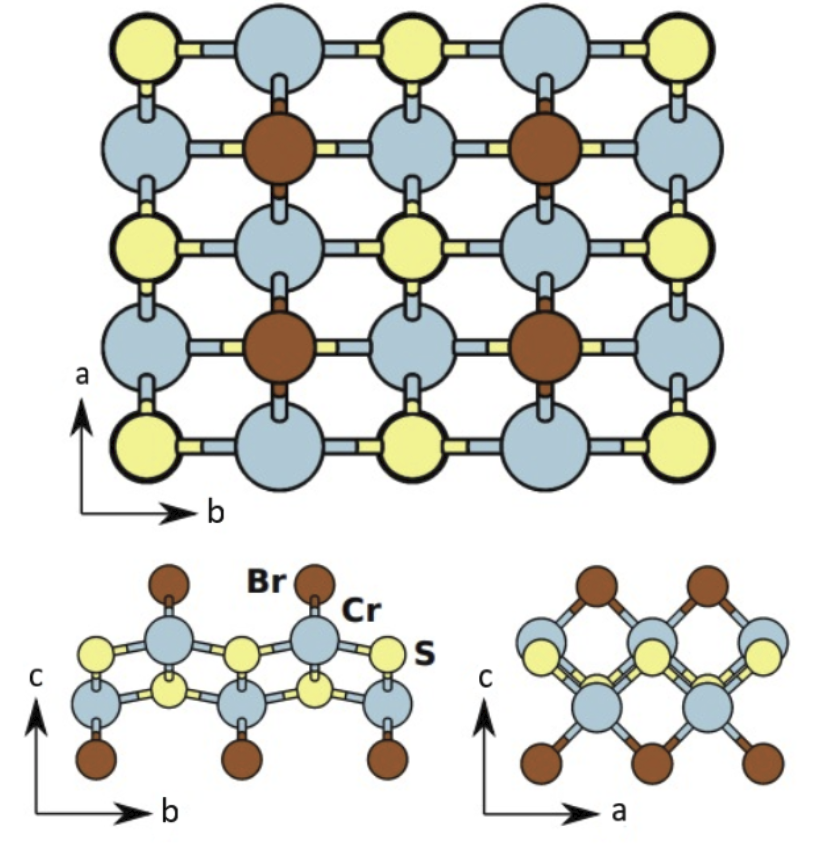
\includegraphics[scale=0.25]{lab2-reticolo.png}
    \caption{Schematic crystal structure of monolayer CrSBr
shown in three different projections. Brown, blue, and yellow balls correspond to Br, Cr, and S atoms respectively.}
    \label{fig:reticolo_sample}
\end{figure}

\noindent CrSBr crystal structure is composed by a succession of layers arranged one on top of the other in the direction \textit{c}. Each one of these layers is made up of a planar structure along directions \textit{a} and \textit{b}. Intralayer bonds are covalent with a certain degree of polarity, due to the not so large difference in electronegativity between the ions, therefore generating a robust intralayer stucture. 
Orthogonally sectioning a single layer it is possible to distinguish a core filled with Chrome and Sulfur ions and an external region where Bromine ions are found, thus generating a pattern Br-(Cr/S)-Br along direction \textit{c}, as shown in Fig. \ref{fig:reticolo_sample}.
Bonds between layers are caused by weak Van Der Waals interactions amongst Bromine ions, which are the outernmost ions in the structure of each layer.
The nature of these bonds makes it easy to exfoliate the crystal, even obtaining monolayers of CrSBr. Our experimental investigation of the magnetic properties of CrSBr have been carried out on a bulk form of the material. $\\$
\noindent DFT calculations and experimental results show that bulk CrSBr is an indirect gap semiconductor characterised by a band gap of 1.42 eV, which is in good agreement with the experimental result (1.5$\pm$0.2 eV). $\\$
\noindent Bulk CrSBr behaves as an A-type antiferromagnet (antiparallel alignment between adjacent layers magnetizations) below its relatively high antiferromagnetic phase transition temperature $T_N$ $\approx$ 132 K. At higher temperatures it is still possible to observe an intralayer ferromagnetic phase, which vanishes over $T_C$ $\approx$ 180 K, leading to a paramagnetic phase of the material. $\\$
\noindent Chrome ions inside the sample are found in a triple ionization configuration Cr$^{3+}$. As a matter of fact, the octahedral lattice potential around Cr ions breaks the fivefold degeneracy of atomic \textit{d} orbitals, causing a splitting of the valence electrons states into \textit{t$_{2g}$} (threefold degenerate) and \textit{e$_g$} (twofold degenerate) states. Since \textit{t$_{2g}$} states are lower in energy, they are more likely to be occupied by electrons, leading to a ground-state configuration in which each \textit{t$_{2g}$} state is partially filled, whereas all of the \textit{e$_g$} states are empty. In order to minimize the on-site repulsion energy, electrons in the valence states arrange in a parallel spin configuration (Hund's Rule), thus generating localized magnetic dipoles on Cr sites in the lattice, related to the total electronic spin state S = 3/2.
Superexchange mechanisms between Cr ions, mediated by S (Cr-S-Cr) or Br (Cr-Br-Cr) ions, produce a ferromagnetic intralayer coupling between the localized magnetic dipoles, which results in a long-range intralayer ferromagnetic ordering. Magnetocrystalline Anisotropy (MA), caused by the presence of spin-orbit coupling, breaks the intraplane isotropy generating an easy-axis of magnetization along direction \textit{b}. The intralayer ferromagnetic phase to paramagnetic phase transition is observed at the Curie temperature $T_C$ $\approx$ 180 K. The interlayer antiferromagnetic magnetization alignment is the result of a super-superexchange mechanism (Cr-Br$\cdots$Br-Cr) between Cr ions belonging to two adjacent layers, mediated by the couple of Br ions interposed between them, which contemplates two possible hopping paths from one Cr ion to the other, as shown in Fig. \ref{fig:supersuperexchange}.

\begin{figure}[h!]
    \centering
    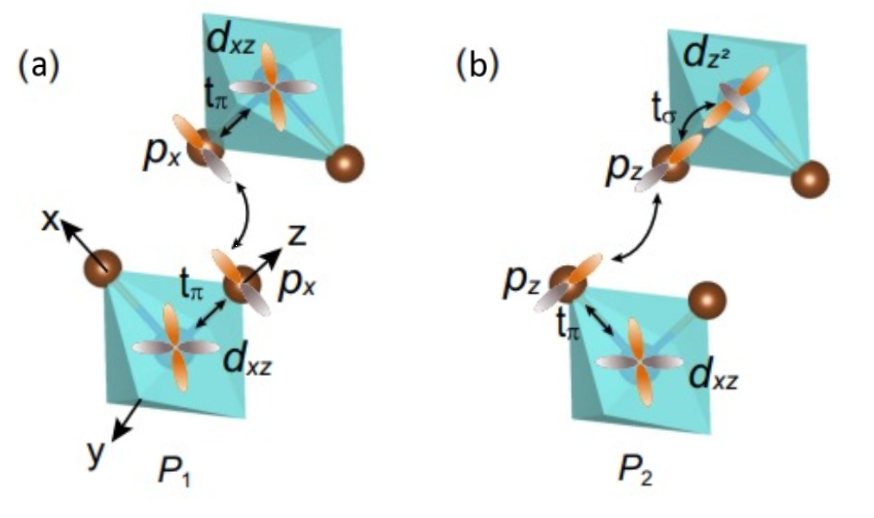
\includegraphics[width=\linewidth]{lab2-supersuperexchange.png}
    \caption{Representation of the two possible hopping paths for the super-superexchange interaction responsible for the interlayer antiferromagnetic alignment.}
    \label{fig:supersuperexchange}
\end{figure}

The path P$_1$ (Fig. \ref{fig:supersuperexchange}.a) represents an interlayer hopping between occupied states on the Cr ions ($d_{xz}$-$d_{xz}$); since both of the orbitals are occupied, hopping is only possible if the interlayer spin alignment is antiferromagnetic. Instead the path P$_2$ (Fig. \ref{fig:supersuperexchange}.b) depicts an interlayer hopping between an occupied state on one Cr ion and an unoccupied state on the other ($d_{xz}$-$d_{z^2}$); in this case hopping is possible for both the interlayer spin ferromagnetic and antiferromagnetic alignments, though the most convenient is the ferromagnetic one because of the Hund's rule. The competition between the antiferromagnetic and ferromagnetic exchange interactions, jointly with the dipole-dipole interaction, which favors an antiparallel alignment, globally results in an antiferromagnetic ground-state of the CrSBr bulk; thus the crystal in its ground-state configuration is an A-type antiferromagnet.
Due to the magnetic dipole-dipole interaction among spin sites in the material, a relevant shape anisotropy (SA) is developed inside the CrSBr crystal. SA is observed when there is a favorable alignment of the localized magnetic dipoles in a certain direction (or directions) which minimizes the total magnetic energy of the system. In our case the advantageous spin alignment results to be along the plane \textit{a}-\textit{b}.
The combined effect of MA and SA leads to a triaxial magnetic anisotropy where \textit{b} is the easy-axis, \textit{a} is the intermediate-axis and \textit{c} is the hard-axis. Rotating the magnetization away from the easy-axis requires the system to pay a certain amount of energy.

\subsection{Synthesis of CrSBr crystals}

The single crystal of CrSBr was synthesized by a Chemical Vapor Transport method (CVT). Cr, S and Br were added and sealed in a terminal of a Quartz tube, in a 1:1:1 molar ratio, under high vacuum and then put into a two zone tube furnace. After a 10h prereaction at 700 °C, which is necessary to vaporize S and Br, the source and growth ends are kept respectively at 850 and 900 °C for 25h in order to allow a reaction between Cr and mixture of S and Br gasses, which lowers Cr vaporization temperature and causes it to turn into its gaseous state.
The last step of the process requires the temperature gradient to be reversed. The source terminal gets slowly heated from 880 to 950 °C over a period of 5 days, while the growth end remains at 850 °C. This allows the vapour to spread towards the growth terminal where it settles, thus forming the crystal.

\section{Experimental Techniques and Setups}

The bulk CrSBr sample was placed on a PCB (Printed Circuit Board) characterized by an elongated shape that allowed us to insert the crystal inside the ESR cavity to carry out the experimental investigations. The sample was welded to the conductive terminals of the PCB, using silver conductive paint and wires, in a way that enabled us to distinguish three connections. By applying an external voltage between two contacts it was possible to establish a collective motion of carriers which could develop either along the layers of the CrSBr crystal or perpendicularly to them. These two schemes were called respectively Current In Plane (CIP) and Current Perpendicular to Plane (CPP) configurations. By choosing different couples of contacts we were able to decide the current direction inside the sample. $\\$
In order to study the magnetic properties of the sample, magnetotransport and ESR measurements were carried out. In the following sections we are going to discuss the different experimental techniques and setups used to perform both types of measurements.

\subsection{Magnetotransport Experimental Setup}

The transport properties of the sample were investigated by observing the variations of the resistance offered by the sample itself to the passage of current in both configurations (CIP and CPP) as a function of the sample temperature and of the applied magnetic field. The sample was inserted in a circuit and an external voltage was applied between two terminals of the sample, using a DC voltage generator, while the current was measured using a picoamperometer connected in series to the sample. The sample was inserted in the ESR cavity in order to exploit the uniform magnetic field produced by the ESR electromagnet and cooled down via a cryostat, which allowed us to control its temperature by adjusting the flux of a cooled N$_2$ gas, that had previously passed through the cryogenic LN$_2$ liquid inside a dewar.

\subsection{ESR Spectroscopy and Setup}

Electron Spin Resonance (ESR) spectroscopy is a method for studying materials that have unpaired electrons. This technique exploits the Zeeman linear splitting of these states ($S\not=0$) depending on the magnitude of the applied magnetic field. By irradiating the system with an electromagnetic radiation at fixed microwave (MW) frequency, it is possible to study the sample absorption of the incoming radiation as a function of the intensity of the applied field.$\\$
The Hamiltonian which describes the coupling between a magnetic dipole $\vec{\mu}$ and a magnetic field $\vec{B}$ is the Zeeman Hamiltonian:

\begin{equation}
    H = - \vec{\mu} \cdot \vec{B}.
\end{equation}

\noindent The magnetic dipole of an electron due to its spin $\vec{S}$ is:

\begin{equation}
    \vec{\mu}=-g\frac{\mu_B}{\hbar}\vec{S}
\end{equation} 

\noindent where $\mu_B$ is the Bohr Magneton and $g$ is called $g$-factor. Since electrons are fermions with S = 1/2, their spin component along the direction of the applied magnetic field could either be $m_s=+\hbar/2$ (spin up) or $m_s=-\hbar/2$ (spin down). For this reason an applied magnetic field $\vec{B_0}$ causes an initially spin degenerate electronic state to be split into two different spin dependent energy levels. The difference in energy between the spin up and spin down states is given by:

\begin{equation}
    \Delta E = E_{\uparrow} - E_{\downarrow} = g\mu_BB_0.
\end{equation}

\noindent When the sample is irradiated with microwaves in resonance with the spin dependent energy splitting of the singly occupied electronic states caused by the static magnetic field $\vec{B_0}$, the coupling between the magnetic dipole of an electron and the radiation magnetic field causes the mixing of the spin up and spin down states along the direction of $\vec{B_0}$, generating electronic transitions from the lower energy spin state to the higher one, which are responsible for the radiation absorption by the sample (provided that the radiation magnetic field has at least a non zero orthogonal component to the static magnetic field).
Probing on a wide range of values of the applied magnetic field it is possible to identify the magnetic field for which the electron states splitting reaches resonance with the incoming radiation. Absorption spectral lines follow a Lorentzian line-shape characterized by a certain linewidth, which depends on electrons lifetime on exited states, in agreement with Heisenberg uncertainty principle. Spin-lattice and spin-spin relaxations are the two main processes that determine the electrons lifetime on the excited states. $\\$
The ESR spectrometer setup is constituted by several fundamental parts, as shown in Fig. \ref{fig:ESR_setupLayout}. 

\begin{figure}[h!]
    \centering
    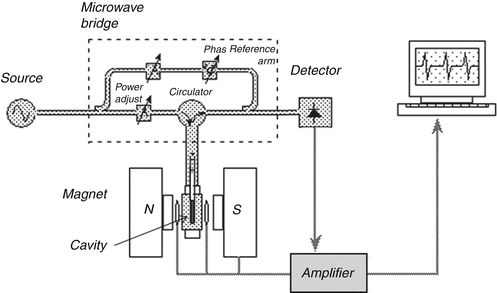
\includegraphics[scale=0.4]{lab2-EPR_setupLayout.png}
    \caption{Main features of an ESR spectrometer. It incorporates a resonant microwave circuit, described as a microwave bridge. The microwave source is a Gunn diode. Perturbation of the microwave radiation is measured by a diode detector.}
    \label{fig:ESR_setupLayout}
\end{figure}

\noindent What follows is a brief discussion about the spectrometer main components:

\subsubsection{Microwave Bridge}

The microwave bridge contains both the microwave source and the detector. The microwave source in modern spectrometers is a Gunn diode, which exploits the Gunn effect, based on the Negative Differential Resistance (NDR) typical of certain semiconductors, to produce microwave radiations with a frequency that can be tuned by coupling the diode to a resonant cavity.
Microwaves emitted by the source pass through a directional coupler which splits the radiation into two paths, the former directed towards the cavity and the latter towards the reference arm. The power of both signals is controlled via a variable attenuator inserted into each of the two paths. The first signal is led to the cavity using a waveguide whilst passing through a circulator. Part of the signal which has reached the cavity may be reflected back depending on the experimental conditions. The use of the circulator is fundamental since it prevents the reflected signal from reaching the source, allowing it through only in the detector direction. The reference signal is then recombined to the reflected signal, using the first as a bias, in order to make the detector diode work in the linear regime of maximum sensitivity. Furthermore, a phase shifter is placed on the reference arm after the attenuator in order to sets a defined phase relationship between the reference and the reflected signal which allows a phase sensitive detection.

\subsubsection{ESR Cavity}

The sample is placed inside the ESR cavity which is essentially a conductive box of a well designed shape that resonates at a tunable microwave frequency. The cavity is utilized to select and stabilize a certain stationary mode of the EM field at a certain frequency in order to distinguish a region where the radiation magnetic field oscillation amplitude is maximized, so that, by placing the sample in the aforementioned region, ESR transitions are encouraged, amplifying the absorption signal coming from the sample. Each resonant cavity is characterized by a Quality Factor Q defined in the following way:

\begin{equation}
    Q = 2\pi\frac{stored \: energy \: inside \: the \: ESR \: cavity}{dissipated \: energy \: per \: microwave \: period}.
\end{equation}

\noindent The stored energy inside the cavity is the total energy associated with the stationary mode of the EM field, while there is always a certain degree of energy dissipation due to resonant and non-resonant sample absorption and induced Eddy currents inside the conductive walls. Since an ESR cavity has an analogous behaviour to that of an RLC resonant circuit, it is possible to express the Q factor as a function of the total impedance of the cavity. Once the resonance condition is achieved and the sample absorbs energy from the radiation, the energy loss inside the cavity peaks, therefore increasing the total cavity impedance. Using an Iris screw, the waveguide and cavity impedances are adjusted to be equal (critically coupled) in a condition in which the microwave frequency is far from resonance with the ESR transitions, hence the reflected power from the cavity in this condition is null. Varying the intensity of the applied magnetic field, the aforementioned condition of resonance is approached and the sample starts absorbing energy, thus increasing the total cavity impedance, losing the condition of critical coupling. At this point the cavity starts to reflect radiation back to the detector, increasing the ESR signal in a way which is proportional to the amount of absorbed power by the sample. In the setup used in the experiment, the ESR cavity was placed inside a cryostat, which utilized an adjustable cooled N$_2$ flux to control the temperature of the sample, monitored by a PID algorithm software. Furthermore the sample was inserted inside a vacuum tube to minimize disturbances that tend to decrease the quality factor Q.

\subsubsection{Signal Detection and Lock-In Amplifier}

The total microwave signal, obtained by the constructive superposition of the reference and the reflected signal, is led to the detector through a waveguide. The detector circuit is an half wave rectifier with capacitor filter, as shown in Fig. \ref{fig:detector-lockInAmp}.a. The oscillating microwave magnetic field passes through an inductor, which converts the EM radiation into AC current. The circuit is thought of in order to turn the incoming current into a DC signal of amplitude equals to that of the AC.

\begin{figure}[h!]
    \centering
    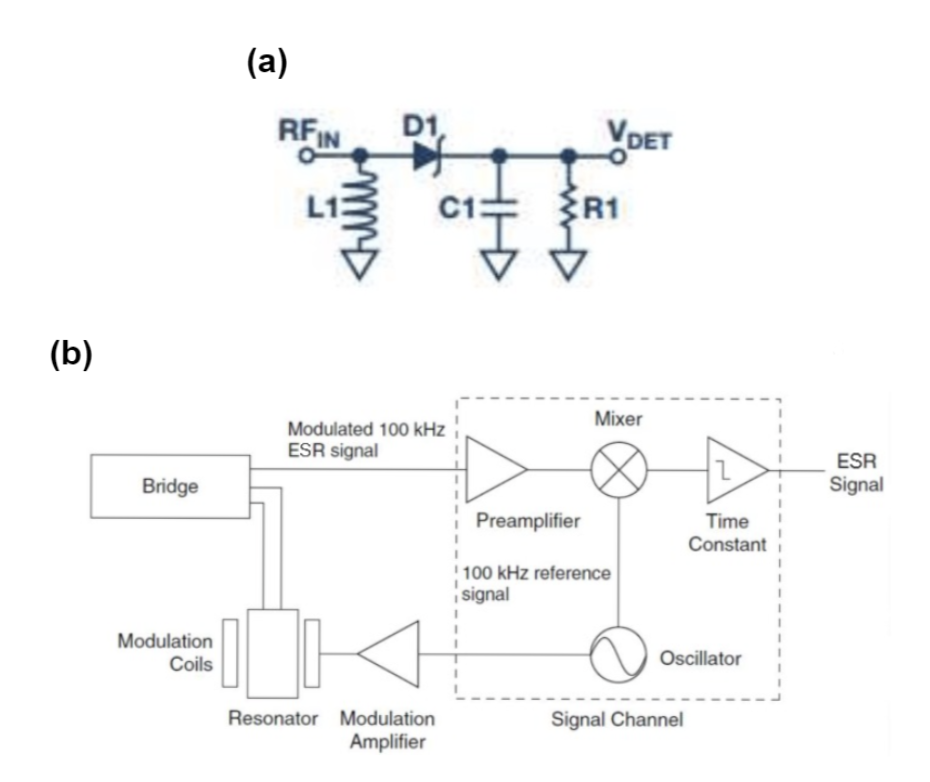
\includegraphics[scale=0.35]{Lab2-diodo_lock-in.png}
    \caption{a) Half-wave rectifier detector with capacitive filter. b) Lock-In Amplifier circuit used to convert the modulated 100 KHz ESR signal into the definitive ESR signal.}
    \label{fig:detector-lockInAmp}
\end{figure}

\noindent The ESR signal $I$ is detected using an additional magnetic field, called Modulation Magnetic Field $\vec{B}_{mod}$, which is produced via suitable modulation coils, located on both sides of the ESR cavity. $\vec{B}_{mod}$ is a sinusoidal field which oscillates in the same direction as the static field $\vec{B}_{0}$ characterized by a frequency fixed at 100 kHz and a modulation amplitude $\Delta B$. The cavity setup is designed in a way which allows the microwave magnetic field to oscillate perpendicularly to $\vec{B}_{0}+\vec{B}_{mod}$. The applied magnetic field oscillation causes the detected signal intensity to fluctuate with the same frequency of the modulation. Suitably pinning $\Delta B$, so that $I(B)$ is linear in the field oscillation range, the intensity of the ESR signal undergoes a sinusoidal modulation whose amplitude is proportional to the first derivative of the intensity itself with respect to the applied static magnetic field: 

\begin{equation}
    \Delta I \simeq \frac{dI}{dB}\Delta B.
\end{equation}

\noindent The modulated ESR signal is exploited as the lock-in amplifier input, as shown in Fig. \ref{fig:detector-lockInAmp}.b, in order to transform it into a DC signal whose amplitude is proportional to its modulation, accordingly obtaining the final first-derivative shaped signal. This transformation process is carried out by mixing the amplifier input signal with a reference 100 kHz sinusoidal one, then cutting out all the high frequency AC components using a low-pass filter. Furthermore, this process cleans the signal from most of the frequency dependent noise, thus improving its quality by increasing the signal-to-noise ratio (SNR).

\section{Data Collection and Analysis}

Our experimental investigation of the properties of a bulk CrSBr sample were realized in two steps. The former had its main focus on the analysis and study of CrSBr magnetotransport characteristics, whereas the latter aimed to highlight and characterize the crystal's properties of anisotropy while also studying its spin dimensionality.

\subsection{CrSBr Magnetotransport}

Before studying the magnetoresistance of the CrSBr crystal it is necessary to observe how the conductance of the sample varies with temperature. The voltage generator was set to provide a 5 V DC tension to the circuit, which was kept fixed throughout the whole experiment. Current measurements were collected for certain temperature steps for both CIP and CPP current configurations. The cryostat used allowed us to reach a minimum temperature slightly lower than 100 K, for this reason our experimental range spanned from 100 K up to room temperature (300 K). Below 180 K a current reading was recorded each time the sample endured a 2 K temperature change, while it was thinned to one every 5 K step once above 180 K. The results of this investigation are shown in Fig. \ref{fig:GvsT}.

\begin{figure*}[h!]
    \centering
    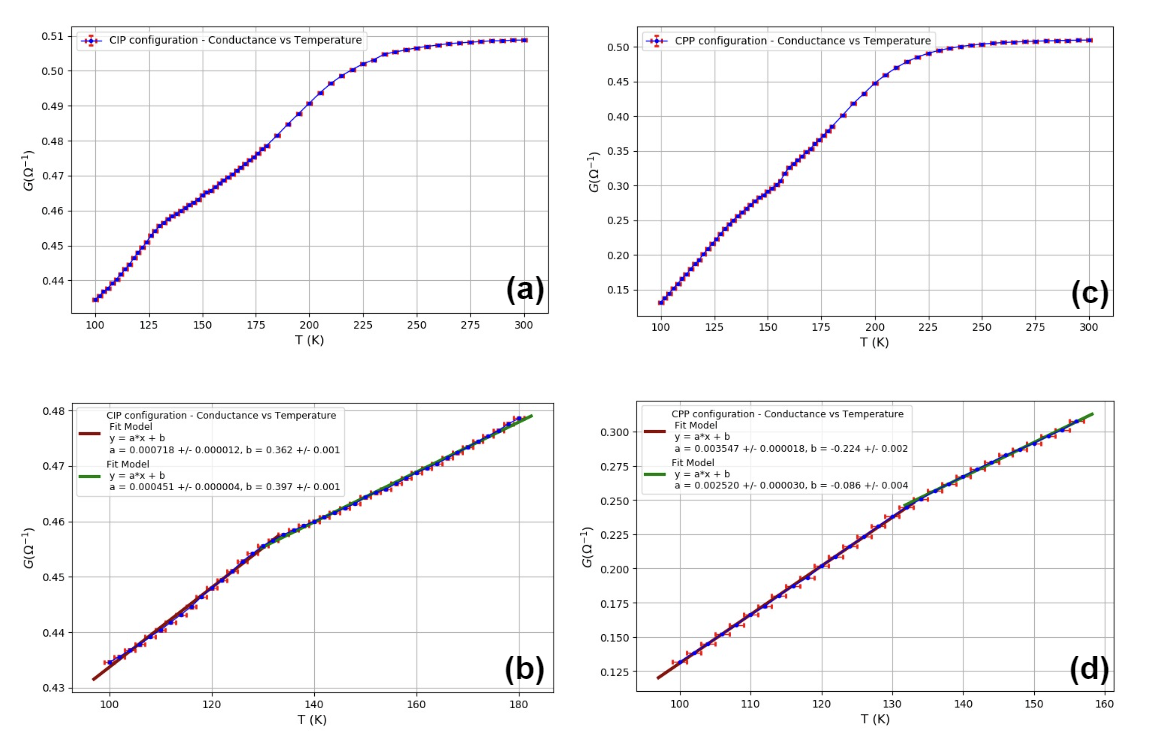
\includegraphics[scale=0.55]{Lab2-GvsT.png}
    \caption{(a) Conductance as a function of the sample temperature in the CIP configuration. (b) Abrupt change of the conductance first derivative with respect to the temperature at T $\approx$ 132 K in the CIP configuration. The $a$ coefficients of the two different fits represent the values of $dG/dT$ at temperatures lower and higher than T = 132 K respectively. (c) Conductance as a function of the sample temperature in the CIP configuration. (d) Abrupt change of the conductance first derivative with respect to the temperature at T $\approx$ 132 K in the CPP configuration. The $a$ coefficients of the two different fits represent the values of $dG/dT$ at temperatures lower and higher than T = 132 K respectively.}
    \label{fig:GvsT}
\end{figure*}

\noindent Conductance was evaluated as $G=\frac{1}{R}=\frac{I}{V}$. Within each reading, an uncertainty of 1 K for the temperature and of 1 nA for the current was estimated. $\\$
\noindent While in a normal conductor it is expected for the conductance to decrease as the temperature increases, due to a larger phonon scattering contribution, in the case of the CrSBr crystal the opposite trend is observed. This behaviour is typical of undoped semiconductors as the carrier concentration increases significantly with temperature. An abrupt change in the conductance first derivative with respect to temperature is observed in both current configurations around $T\simeq132 K$. The slope decreases at this temperature by approximately 37\% in the CIP configuration, and by 29\% in the CPP configuration. This rapid variation can be interpreted as the onset of the antiferromagnetic interlayer ordering. This allows us to identify the temperature at which the kink in conductance is observed with the Néel temperature $T_N$. In a single ferromagnetic layer there is an nonequivalent distribution of electrons in the spin resolved semiconductor band structure that leads to a different spin resolved density of states at the Fermi level, which causes the scattering probability to depend on spin. Below Néel temperature the layers magnetization alignment is antiparallel, thence resulting in a high-resistivity state for both spin channels in the easy-axis direction, therefore diminishing conductance more rapidly as temperature decrease below $T_N$.
\noindent It is then possible to observe the magnetoresistance effects on the sample by varying the applied magnetic field intensity. Our investigation focused on studying these effects in the CIP configuration with the magnetic field along the easy-axis \textit{b}. During the experiment the magnetic field intensity was varied from 0 to 7000 G in steps of 50 G. Using a picoamperometer, for each value of the applied magnetic field, the current intensity was registered and then used in order to evaluate the resistance of the sample. The percentage magnetoresistance has also been calculated, referring to the resistance measured at zero magnetic field, using the following formula:

\begin{equation}
    MR(\%) = \frac{R(B)-R(0)}{R(0)}\times100
\end{equation}

\noindent This process was carried out at both 100 K and 132 K separately, so that a comparison between the sample magnetoresistance below and around Néel temperature $T_N$ could be drawn. Experimental results are shown in Fig. \ref{fig:MR_at_T}.

\begin{figure*}[h!]
    \centering
    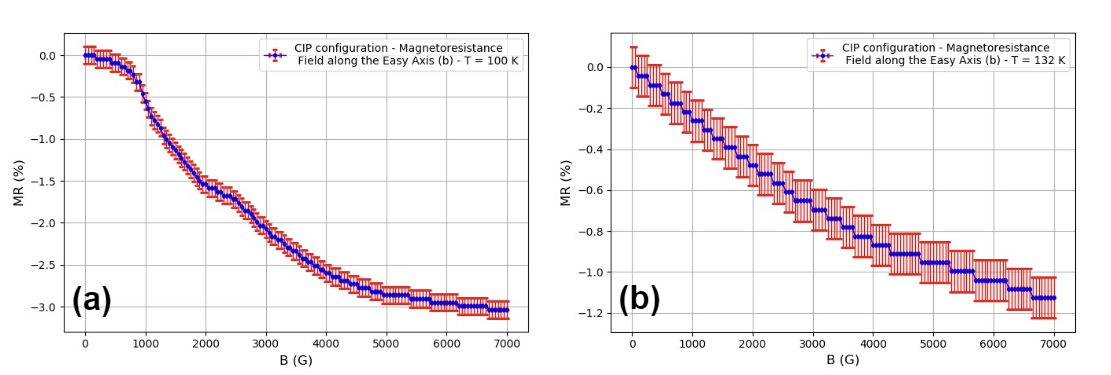
\includegraphics[width=\linewidth]{MR_at_T.png}
    \caption{Magnetoresistance effects measured on the sample at 100K (a) and 132K (b) in the CIP configuration, with the magnetic field aligned along the easy-axis \textit{b}.}
    \label{fig:MR_at_T}
\end{figure*}

\noindent Both pictures show the presence of a negative magnetoresistance (nMR) effect due to the layers magnetization alignment in the magnetic field direction. If the sample temperature is less than $T_N$, the adjacent layers magnetization alignment is antiparallel for low magnetic field intensities. This antiferromagnetic configuration hinders interlayer tunneling. By increasing the magnetic field along the easy-axis of magnetization in a defined direction, the layers magnetizations which are initially antiparallel to the applied field are gradually reversed, therefore producing a configuration of complete parallel alignment of the layers magnetic dipoles. This effect causes an alteration of the spin-dependent scattering in the layers where the magnetization is reversed which results in the decrease of the resistivity of one of the spin channels. In this configuration interlayer tunneling is encouraged, thus reducing the sample resistivity with respect to the zero applied field condition.
Once the applied field is intense enough, it is possible to observe that the sample resistance remains approximately constant by increasing the field strength even more. This last effect is called saturation and it is related to the achievement of maximum parallel alignment of the layers magnetizations in the direction of the applied field. The lowest applied magnetic field intensity which fully develops this condition is called saturation magnetic field $B_S$. Analyzing the magnetoresistance of the CrSBr sample at 100 K shown in Fig. \ref{fig:MR_at_T}.a it is possible to notice a sudden flattening of the magnetoresistance trend at approximately 5000 G, which can be interpreted as the saturation field $B_S$ in this condition, since significant variations in the magnetoresistance cannot be identified once exceeded this value. 
The magnetoresistance value measured is around $-3,0\%$ at 100 K.
If the sample temperature is greater than $T_N$ the antiferromagnetic ordering of the adjacent layers magnetizations is lost, thus the magnetoresistance exhibited by the sample when the interlayer ferromagnetic ordering is established through the application of a magnetic field is notably reduced. An evidence of this effect may be observed in Fig. \ref{fig:MR_at_T}.b, where an important reduction in the nMR value can be noticed (approximately $1/3$ of the previously discussed case at 100 K). Another relevant feature that can be noticed in the previous trend is the absence of a saturation effect in the MR, since only a decrease in its slope is recorded at high magnetic field intensities. This phenomenon could be related to the presence of a higher concentration of spin-wave excitations, originated by the different temperature regime, which hinders the establishment of a fully ferromagnetic aligned spin system. Eventually, referring to other research results, a lower than expected MR value has been obtained both at 100 K and 132 K. Even though the MR effects are still observable, there could have been some issues related to the setup, in particular with the soldering and etching of the sample, which are the only two processes that were conducted by hand, which could have translated in a modification of the sample behaviour. For the sake of fairness the whole experiment should be conducted again in order to obtain a new set of data from a different sample that could both validate or not the quantitative results previously showcased.

\subsection{CrSBr Anisotropy}

Here follows a description of the settings choosing and analysis procedure used during the ESR experiment to investigate the anisotropy and spin dimensionality of the crystal:

\subsubsection{ESR Parameters Setting}

An ESR spectrometer gives the possibility to set certain amount of parameters. The main focus is to choose the right value for each parameter in order to obtain the best experimental outcomes. This section will discuss some of these settings and the motivations behind the choices made. The magnetic field run experiment is executed with a sweep width of 4000 G, starting from a value of 1351 G up to 5351 G in a time (sweep time) of 20,97 s. These two parameters are to be considered as fixed in our experimental setup.
Once these two parameters have been chosen, the next one to set is the time constant of the spectrometer, which corresponds to the characteristic time of the low-pass filter present in the lock-in amplifier as represented in fig. \ref{fig:detector-lockInAmp}.b. Since a very high time constant tends to filter part of the signal, while a too low time constant leads to an excessively noisy one, it is important to find the optimal value that allows to optimize the SNR without causing distortions to the signal itself. Time constant can be chosen in the optimal way using the following formula:

\begin{equation}
    time \; constant = \frac{linewidth}{sweep \; width} \times sweep \; time \div 10
\end{equation}

\noindent Executing a tryout running with default ESR parameters, it is possible to measure the linewidth (peak-to-peak field difference) which can be used to evaluate the optimal time constant. In our case, running a preliminary test, we obtained a linewidth of the order of 220 G, which translates in an optimal time constant approximately equal to 115 ms. Since the ESR spectrometer only permits the selection of the time constant value inside a discrete set, the best possible choice that can be made consists in the closest allowed value to the optimal one, which in our case was 163.84 ms. Accordingly adjusting the time constant, the quality of the signal improved reasonably when compared to the first test, which was carried out using a time constant equal to 20.48 ms. This improvement is evidenced by a 11.1\% increase in the SNR. $\\$
\noindent The remaining parameters to discuss are the magnetic field modulation amplitude (MA) and the MW attenuation (or equivalently MW power). Setting an MA too small causes the signal to be weak, thus making the electrical noise extremely influential in the ESR spectra analysis, while setting it too large causes the ESR signal to be distorted, since in this case the magnetic field oscillation spans a large interval in which the signal intensity ceases to be linear. In order to choose the MA appropriately, it is necessary to run a series of tests in which the MA is varied while keeping the other parameters fixed. In this case the investigation was carried out starting from the default value of 5.00 G, increasing it to 10.00 G and then 19.67 G. The spectral linewidth results to be unchanged, within the limits of uncertainty, while the peak-to-peak intensity difference shows a linear increase when plotted as a function of the MA in the analyzed interval. Since in all the tests performed the signal was sufficiently intense and the peak-to-peak intensity difference followed the aforesaid trend, which witnessed a lack of distortion in the scanned interval, it was possible to randomly choose one of the permitted values without any kind of distinction whatsoever. We decided to use the MA default value because it resulted in the best possible SNR value. Regarding MW attenuation a series of measurements have been conducted varying its value while keeping every other parameter constant. The peak-to-peak intensity of an ESR signal increases linearly with the square root of the microwave power in the absence of saturation effects. When saturation sets in, the signal broadens causing the peak-to-peak intensity to decrease while the linewidth increases, leading to an effective distortion. The results of this investigation are reported in Fig.\ref{fig:MW_Power}. 

\begin{figure}[h!]
    \centering
    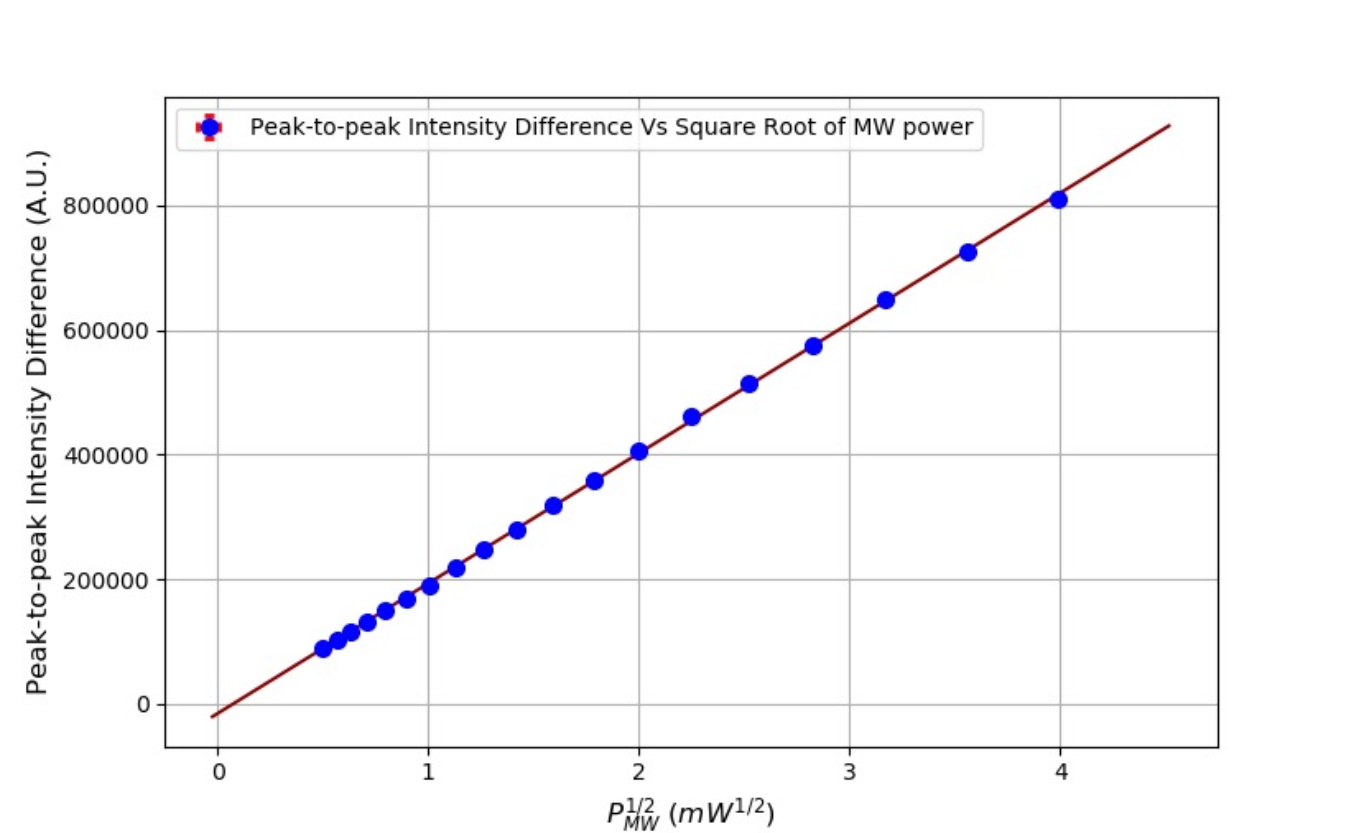
\includegraphics[width=\linewidth]{Lab2-MW_Power.png}
    \caption{Peak-to-peak intensity difference vs square root of MW power plotted with linear fit.}
    \label{fig:MW_Power}
\end{figure}

\noindent In the scanned MW power interval, starting from an attenuation of -29 dB (0.25 mW) up to -11 dB (16 mW), it is possible to observe that the peak-to-peak intensity difference maintains a linear trend. We decided to set the MW attenuation to -20 dB, which corresponds to a MW power of 2.00 mW, so that this value of attenuation prevents us from saturation while also providing a sufficiently strong signal.

\subsubsection{ESR Results Analysis}

The investigation objective is to prove the spin dimensionality of the bulk CrSBr sample meanwhile observing and quantifying the crystal spatial anisotropy. At room temperature (295 K) the sample was placed inside the ESR cavity in the out-of-plane configuration, as shown in Fig. \ref{fig:out-of-plane}. In this configuration the ESR magnetic field is always applied orthogonally to the \textit{a} axis along a direction which forms an angle $\theta_B$ with respect to the \textit{b} axis. 

\begin{figure}[h!]
    \centering
    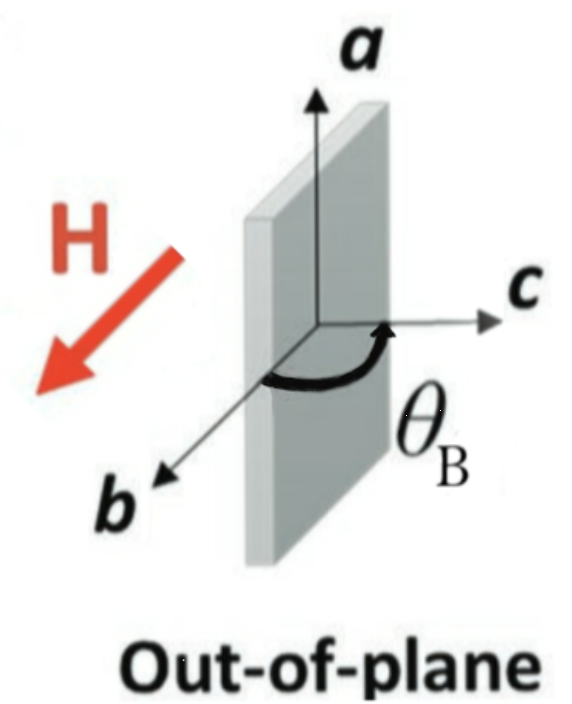
\includegraphics[scale=0.25]{out-of-plane.png}
    \caption{Representation of the out-of-plane configuration used for the ESR angular dependent investigation and the definition of the angle $\theta_B$.}
    \label{fig:out-of-plane}
\end{figure}

\noindent A multitude of ESR spectra were recorded rotating the sample with steps of $2^{\circ}$ from $\theta_B=0^{\circ}$ to $\theta_B=180^{\circ}$. The sample rotation process was carried out using an E-229 protractor, equipped with a graduated scale. By sampling the variations of the resonance field intensity $B_{res}$ and the spectral linewidth $\Delta B$ with the rotation of the sample it is possible to determine and quantify the out-of-plane magnetic anisotropy constant $K_{\bot}$, the variation in the Cr$^{3+}$ effective magnetic dipole in the \textit{b}-\textit{c} plane and the spin dimensionality of the system.
The magnetic resonance field intensity and the spectral linewidth for each sample angular configuration were estimated from the corresponding spectrum respectively by determining the field intensity which cancelled the ESR signal between the positive and negative peaks and by measuring the peak-to-peak field difference.
The results of this investigation are summarized in Fig. \ref{fig:ESR_Results}.


\begin{figure*}[h!]
    \centering
    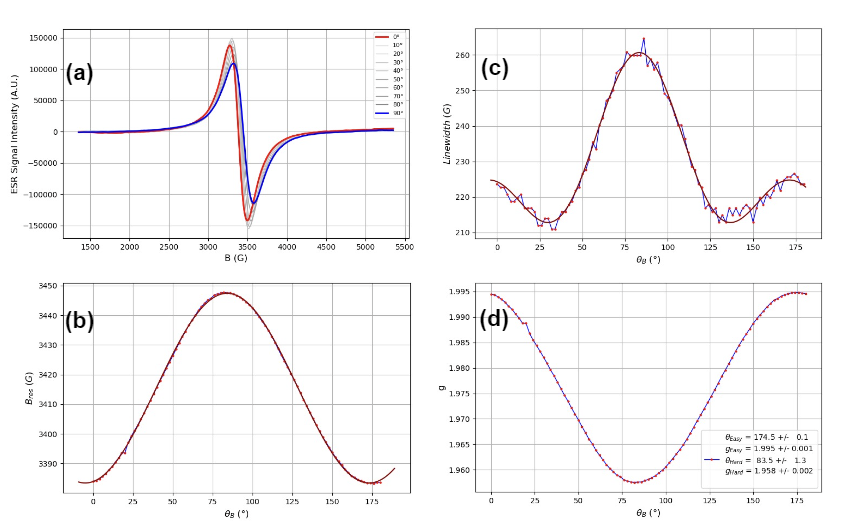
\includegraphics[width=\linewidth]{Lab2-Resonance.png}
    \caption{(a) Evolution of the ESR spectrum observed by rotating the sample in the out-of-plane configuration in steps of $10^{\circ}$ from $\theta_B=0^{\circ}$ (ESR field approximately aligned along \textit{b}) up to $\theta_B=90^{\circ}$ (ESR field approximately aligned along \textit{c}). 
    (b) Resonance magnetic field $B_{res}$ dependence on the sample angular orientation $\theta_B$ in the out-of-plane configuration.
    (c) Linewidth $\Delta B$ dependence on the sample angular orientation $\theta_B$ in the out-of-plane configuration. The function model utilized to fit the W-like shaped experimental data is reported in the Appendix in Sec. B.
    (d) Cr$^{3+}$ electrons \textit{g}-factor angular dependence in the \textit{b}-\textit{c} plane.}
    \label{fig:ESR_Results}
\end{figure*}

\noindent Once the $B_{res}$ out-of-plane angular dependence is obtained, the corresponding magnetic anisotropy constant can be calculated through the use of the following formula:

\begin{equation}
    K_{\bot} = \frac{1}{2}M_sB_{i\bot}.
    \label{eq:AnisotropyConstant}
\end{equation}

\noindent $M_s$ is the saturation magnetization of the sample, estimated to be equal to $0.48$ T in other experiments, and $B_{i\bot}$ is the perpendicular internal anisotropy field, which corresponds to the difference between the maximum and minimum value of the recorded resonance magnetic field $B_{res}$. $K_{\bot}$ represents the spatial energy density needed to rotate the crystal magnetization from the easy-axis to the hard-axis. From the constants A and C obtained from the fitting function of the resonance magnetic field trend depending on the angle $\theta_B$, represented in the equation (\ref{eq:B_res_fit}) reported in Sec. B of the Appendix, it was possible to evaluate the offset magnetic field and the perpendicular internal anisotrpy field, eventually obtaining the following results: $B_{0\bot}=(3.3834\pm0.0001)\cdot10^3\:$G, $B_{i\bot}=(6.40\pm0.01)\cdot10^1\:$G.
\noindent Using Eq. (\ref{eq:AnisotropyConstant}), the value obtained for the perpendicular anisotropy constant is $K_{\bot}=(1.536\pm0.003)\cdot10^{-3}$ T$^2 = (1.222\pm0.002)\cdot10^3$ J$\cdot$m$^{-3}$. $\\$
In order to underline this anisotropy we focus on the evaluation of the Cr$^{3+}$ unpaired electrons \textit{g}-factor. Typically unpaired electrons occupying energy states inside a crystal are characterized by an effective \textit{g}-factor which differs from the free electron value $g_e$ whilst also being anisotropic. Applying an external magnetic field on a crystal, an electron inside the crystalline environment does not only interacts with the external field $\vec{B}_0$, but also with the local field $\vec{B}_{loc}$, which comprehends the induced or intrinsic magnetization, together with a whole set of other contributes mainly related to the Spin-Orbit Coupling (SOC) and to the Ligand Crystal Field (LF). For this reason an effective \textit{g}-factor expressed in a second order tensor form can be introduced to describe the interaction of the electron with the total magnetic field $\vec{B}_{0} + \vec{B}_{loc}$ as if the electron is only coupled to the external magnetic field $\vec{B}_{0}$:

\begin{equation}
    H = g_e\frac{\mu_B}{\hbar}(\vec{B}_0+\vec{B}_{loc})\cdot\vec{S} = \frac{\mu_B}{\hbar}\vec{B}_0\cdot\vec{\vec{g}}\cdot\vec{S}.
\end{equation}

\noindent The SOC tends to deviate the value of the effective \textit{g}-factor from $g_e$, whereas the LF tends to reflect its symmetry on the induced magnetization and electron \textit{g}-tensor, thus producing its characteristic anisotropy. $\\$
\noindent The \textit{g}-tensor can be investigated via the angle-dependent ESR spectra. Firstly it is necessary to note that, as a 3x3 Hermitian tensor, the \textit{g}-tensor can be diagonalized through the appropriate choice of the Cartesian reference system. In the case of CrSBr the choice involves the use of the reference system composed by the easy, intermediate and hard axes. It is expected that the \textit{g}-factor is maximum along the crystal easy-axis of magnetization and minimum along the crystal hard-axis of magnetization.
The resonance condition is achieved inside the crystal when the superposition of the applied and internal fields generates a energy splitting of the electrons states which equals the incoming photon frequency. Since on the easy-axis a larger response from the system is achieved in terms of magnetization intensity, the applied field magnitude which realizes the resonance diminishes, whereas the opposite happens in the hard axis direction. For this reason, when the electrons \textit{g}-factor is calculated an plotted depending on the orientation of the crystal, it is possible to identify the crystal easy-axis and hard-axis with the directions which maximize and minimize \textit{g} respectively. Based on how it is defined, \textit{g} can be calculated from the ESR parameters via the following relation:

\begin{equation}
    h\nu = g\mu_BB_{res} \:\: \Longrightarrow \:\: g = \frac{h\nu}{\mu_BB_{res}}
\end{equation}

\noindent The results of the out-of-plane investigation of the Cr$^{3+}$ unpaired electrons \textit{g}-factor are shown in Fig. \ref{fig:ESR_Results}.d. Since the photon energy $h\nu$ is kept fixed, there is an inverse proportionality relationship between \textit{g} and $B_{res}$. From the previous considerations it is possible to identify the easy-axis of magnetization with the \textit{b} axis since the maximum value of \textit{g} is recorded at an angle $\theta_B = (174.5\pm0.1)^{\circ}$ and coincides with the value of $g_{easy}=1.995\pm0.001$, whilst the hard-axis of magnetization can be identified with the \textit{c} axis since the minimum value of \textit{g} is recorded at an angle $\theta_B = (83.5\pm1.3)^{\circ}$ and coincides with the value of $g_{hard}=1.958\pm0.002$. The $6^{\circ}$ deviation from the expected $\theta_B=0^{\circ}$ for the easy-axis and $\theta_B=90^{\circ}$ for the hard-axis is probably due to irregularities in the crystal layers parallel alignment with the PCB surface on which it was welded.
Utilizing the \textit{g}-factor values in the easy and hard axis directions obtained, it is possible to evaluate the Cr$^{3+}$ ion magnetic moment via the following formula:

\begin{equation}
    \mu = g\sqrt{S(S+1)}\mu_B.
\end{equation}

\noindent The ions magnetic moment can be evaluated via the spin state $S=3/2$ only since electrons occupying \textit{d}-orbitals inside a crystal show a quenched orbital angular momentum, which weakly contribute to the total angular momentum state and consequently to the magnetic dipole of the ion.
The orbital angular momentum quenching is caused by the interaction of the valence electron with the crystal field, which causes the valence \textit{d}-orbitals to be split. Since the resulting states are obtained as a linear combination of the atomic \textit{d}-orbitals, they are generally no longer eigenstates of the orbital angular momentum component along the direction of the applied magnetic field. For this reason, the aforementioned component is no longer a constant of motion and it averages to zero, canceling the contribution of the electron orbital angular momentum to the ion magnetic moment.
The experimental values of the Cr$^{3+}$ effective magnetic moment on the easy and hard axis are $\mu_{easy}=(3.863\pm0.004)\mu_B$ and $\mu_{hard}=(3.791\pm0.004)\mu_B$ respectively, averaging to $\bar{\mu}_{\bot}=(3.827\pm0.004)\mu_B$, which is in agreement with the expected magnetic moment of a Cr$^{3+}$ ion with quenched orbital angular momentum. $\\$
Once the out-of-plane crystal anisotropy has been observed and quantified, through the same ESR investigation it is also possible to determine the spin dimensionality of the crystal. This procedure is carried out by observing that the optimal fitting function of the ESR spectral linewidth angular dependence is performed using Eq. (\ref{eq:linewidth_fit}), reported in Sec. B of the Appendix, which describes well the W-like shape of the linewidth trend. This peculiar shape is characteristic of two-dimensional magnets and it is significantly different from the linewidth angular dependence of three-dimensional magnets, which shows a V-like shape.
The ESR spectral linewidth angular dependence is critically related to the spin-spin relaxation mechanism, which is strongly influenced by spin-spin correlations. Bulk CrSBr at room temperature is expected to be in its paramagnetic phase since $T_C\approx180K$, but the linewidth angular dependence shows that spin-spin correlations are still present since the trend followed is a W-shape one. The fact that bulk CrSBr crystals show this behaviour even at room temperature means that spin-spin correlations are not yet disrupted by spin wave excitations, which means that there is a substantial gap in the spin wave excitation DOS spectrum. This behaviour can only be interpreted via the XY-model for a two-dimensional magnet.
The same trend of the linewidth angular dependence has been observed in many other two-dimensional magnets, particularly at low temperatures.

\section{Conclusions}

From the magnetotransport measurements, we conclude that the electrical properties of bulk CrSBr are strongly coupled to the magnetic order. The observed negative magnetoresistance is a direct result of the layered antiferromagnetic structure of CrSBr. The magnetotransport results obtained are qualitatively in good agreement with other experimental results and can be correctly interpreted using theoretical predictions, even though they are significantly different from the quantitative point of view. Therefore a new magnetotransport investigation is suggested in order to obain more reliable results. $\\$
Via the ESR investigation at room temperature it was possible to observe and study the bulk CrSBr crystal anisotropy, evaluating the magnetic anisotropy constant in the out-of-plane configuration and also the angular \textit{g}-factor dependence, while simultaneously probing the spin dimensionality of the system. Regarding the last point, the W-shaped ESR linewidth angular dependence can be explained in terms of the XY-model, which applies for two-dimensional magnets. 
Eventually the whole study conducted can be deemed as moderately successful.

\appendix

\subsection{SNR Evaluation}
In a single spectrum acquisition process it is of the utmost importance to calculate the Signal-To-Noise Ratio (SNR) to quantify the signal quality.
The signal is estimated to be equal to the maximum intensity peak recorded in the whole ESR spectrum, while the noise is estimated from the standard deviation of the intensity values recorded in the region where the ESR signal is flat, which means taking into account the magnetic field intervals of the spectrum which are far from resonance.

\subsection{ESR Angular Dependence Fitting Models}

The resonance magnetic field $B_{res}$ shows an oscillating behaviour as a function of $\theta_B$ which has been fitted to the following function:

\begin{equation}
    B_{res\bot} (\theta_B) = A + C\cos^2(\theta_B + \phi)
    \label{eq:B_res_fit}
\end{equation}

\noindent which has a $\pi$ periodicity. A and C are the two relevant fitting constant through which the offset field $B_{0\bot}$ and the perpendicular internal anisotropy field $B_{i\bot}$ can be obtained. $\\$
\noindent The linewidth shows a W-like shaped behaviour as a function of $\theta_B$ which has been fitted to the following function:

\begin{equation}
    \Delta B (\theta_B) = \frac{F}{4}(\cos^2(\theta_B + \Phi)-1)^2 + G
    \label{eq:linewidth_fit}
\end{equation}

\noindent which has a $\pi$ periodicity.

\twocolumn[
  \begin{@twocolumnfalse}
     \nocite{*}
     \bibliographystyle{unsrtnat}
     \bibliography{Biblio.bib}
   \end{@twocolumnfalse}]
\thispagestyle{empty}

\end{document}